\begin{figure}[htbp]
\centering
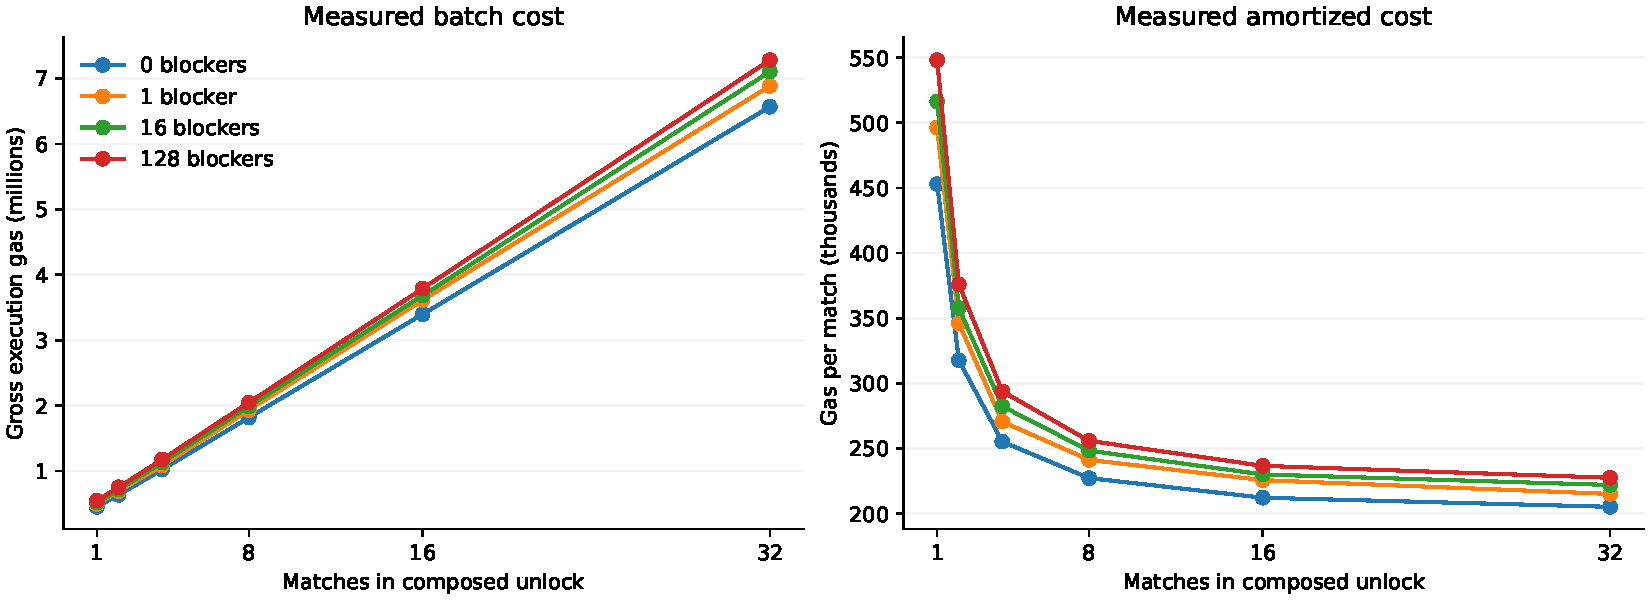
\includegraphics[width=\textwidth]{figures/eligible-gas.pdf}
\caption{Measured gross execution gas; 32 resting sells and buys, zero to 128 ineligible high-fee asks.}
\end{figure}
\begin{center}
\begin{tabular}{r r r r r}
\hline
Matches & 0 blockers & 1 blocker & 16 blockers & 128 blockers \\
\hline
1 & 452,954 & 496,378 & 516,326 & 548,122 \\
2 & 635,406 & 692,152 & 715,453 & 751,862 \\
4 & 1,021,021 & 1,082,234 & 1,129,693 & 1,175,342 \\
8 & 1,818,257 & 1,930,212 & 1,986,830 & 2,047,008 \\
16 & 3,395,491 & 3,611,461 & 3,681,130 & 3,786,877 \\
32 & 6,567,163 & 6,883,944 & 7,103,759 & 7,280,650 \\
\hline
\end{tabular}
\end{center}
The benchmark measures a real hook/PoolManager unlock after cooling storage accessed by a
dry run. Values are gross execution gas around the test-harness unlock, without storage
refund subtraction or transaction intrinsic gas. Standard ERC-20 fixtures and no active LP
positions are used. Rows above eight matches compose multiple matching calls inside that
unlock; they do not describe a new Router batch endpoint. The largest tested batch is 32,
not a demonstrated global optimum. The 128-blocker example is not the worst possible
128-branch trie shape. At eight matches its measured cost is 2,047,008 gas; at 32 it is
7,280,650 gas, or about 227,520 gas per match. A gas budget and a certified external-call
envelope are still needed before increasing a production per-call cap.
